\documentclass{standalone}
\usepackage{tikz}
\begin{document}
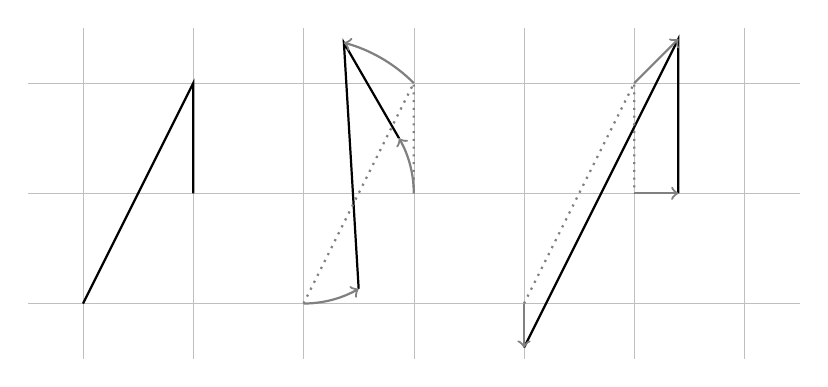
\begin{tikzpicture}[fill=gray,thick,scale=1.4]
\draw[step=1,gray!50!white,very thin] (0.5,0.5) grid (7.5,3.5);

\draw[xshift=1cm,yshift=2cm] (0,-1) -- (1,1) -- (1,0);

\begin{scope}[xshift=3cm,yshift=2cm] % can move path actions to scope
    \begin{scope}[rotate=30]
        \draw (0,-1) -- (1,1) -- (1,0);
    \end{scope}
    \begin{scope}[gray,dotted]
        \draw (0,-1) -- (1,1) -- (1,0);
    \end{scope}
    \begin{scope}[gray,->]
        \draw (0,-1) arc (270:300:1);
        \draw (1,1) arc (45:75:1.41421);
        \draw (1,0) arc (0:30:1);
    \end{scope}
\end{scope}

\begin{scope}[xshift=5cm,yshift=2cm]
    \begin{scope}[scale=1.4]
        \draw (0,-1) -- (1,1) -- (1,0);
    \end{scope}
    \begin{scope}[gray,dotted]
        \draw (0,-1) -- (1,1) -- (1,0);
    \end{scope}
    \begin{scope}[gray,->]
        \draw (0,-1) -- (0,-1.4);
        \draw (1,1) -- (1.4,1.4);
        \draw (1,0) -- (1.4,0);
    \end{scope}
\end{scope}

\end{tikzpicture}
\end{document}
